\documentclass[aspectratio=169, 14pt]{beamer}
\usepackage[utf8]{inputenc}
\usepackage{xeCJK}
\usepackage{tipa}
\usepackage{graphicx}
\usepackage{transparent}
\usepackage[ruled, lined, linesnumbered, commentsnumbered]{algorithm2e}
\usepackage{tikz}
\usetikzlibrary{calc,shadows.blur}
\usetikzlibrary{matrix,backgrounds}
\usetikzlibrary{arrows, positioning}
\usepackage{minted}
\usepackage{fontawesome5}
\usepackage{booktabs}
\usepackage{hyperref}
\hypersetup{
    colorlinks=true,
    linkcolor=blue,
    filecolor=magenta,      
    urlcolor=cyan,
    }
\urlstyle{same}
\usetheme{metropolis}
\metroset{block=fill}
\usecolortheme{default}
\definecolor{darkmidnightblue}{rgb}{0.0, 0.2, 0.4}
\definecolor{LightGray}{gray}{0.9}
\definecolor{usecolor}{RGB}{141,143,168}
\newcommand\grid[1]{%
\fontsize{80}{80}
\begin{tikzpicture}[baseline=(char.base)]
  \path[use as bounding box]
    (0,0) rectangle (1em,1em);
  \draw[help lines,step=0.5em]
    (0,0) grid (1em,1em);
  \draw[help lines,dashed]
    (0,0) -- (1em,1em)  (0,1em) -- (1em,0);
  \node[inner sep=0pt,anchor=base west]
    (char) at (0em,\gridraiseamount) {#1};
\end{tikzpicture}}                                                                                                                       
% \gridraiseamount is a font-specific value
\newcommand\gridraiseamount{0.12em}

%------------------------------------------------------------
%This block of code defines the information to appear in the
%Title page
\title[Database Principles and Applications] %optional
{数据库原理与应用}

\subtitle{课程介绍}

\author[CHEN Zhongpu] % (optional)
{CHEN Zhongpu}

\institute[] % (optional)
{
  School of Computing and Artificial Intelligence \\
  \href{mailto:zpchen@swufe.edu.cn}{zpchen@swufe.edu.cn}
}

\date[] % (optional)
{SWUFE, Fall 2022}

%End of title page configuration block
%------------------------------------------------------------


%------------------------------------------------------------
%The next block of commands puts the table of contents at the 
%beginning of each section and highlights the current section:

% \AtBeginSection[]
% {
%   \begin{frame}
%     \frametitle{Table of Contents}
%     \tableofcontents[currentsection]
%   \end{frame}
% }
%------------------------------------------------------------


\begin{document}

%The next statement creates the title page.
\frame{\titlepage}

%---------------------------------------------------------
%This block of code is for the table of contents after
%the title page
% \begin{frame}
% \frametitle{Table of Contents}
% \tableofcontents
% \end{frame}
%--------------------------------------------------------
\begin{frame}
    \frametitle{关于我:陈中普}
    
    \begin{block}{\faIcon{book} 研究方向}
        时空数据库,大数据分析
    \end{block}
    
    \begin{block}{\faIcon{building} 办公室}
        通博楼B-422
    \end{block}
    
    \begin{block}{\faIcon{home} 主页}
        \href{https://zhongpu.info}{https://zhongpu.info}
    \end{block}
    
\end{frame}

{
    % \usebackgroundtemplate{\transparent{0.3}{\begin{picture}
    %     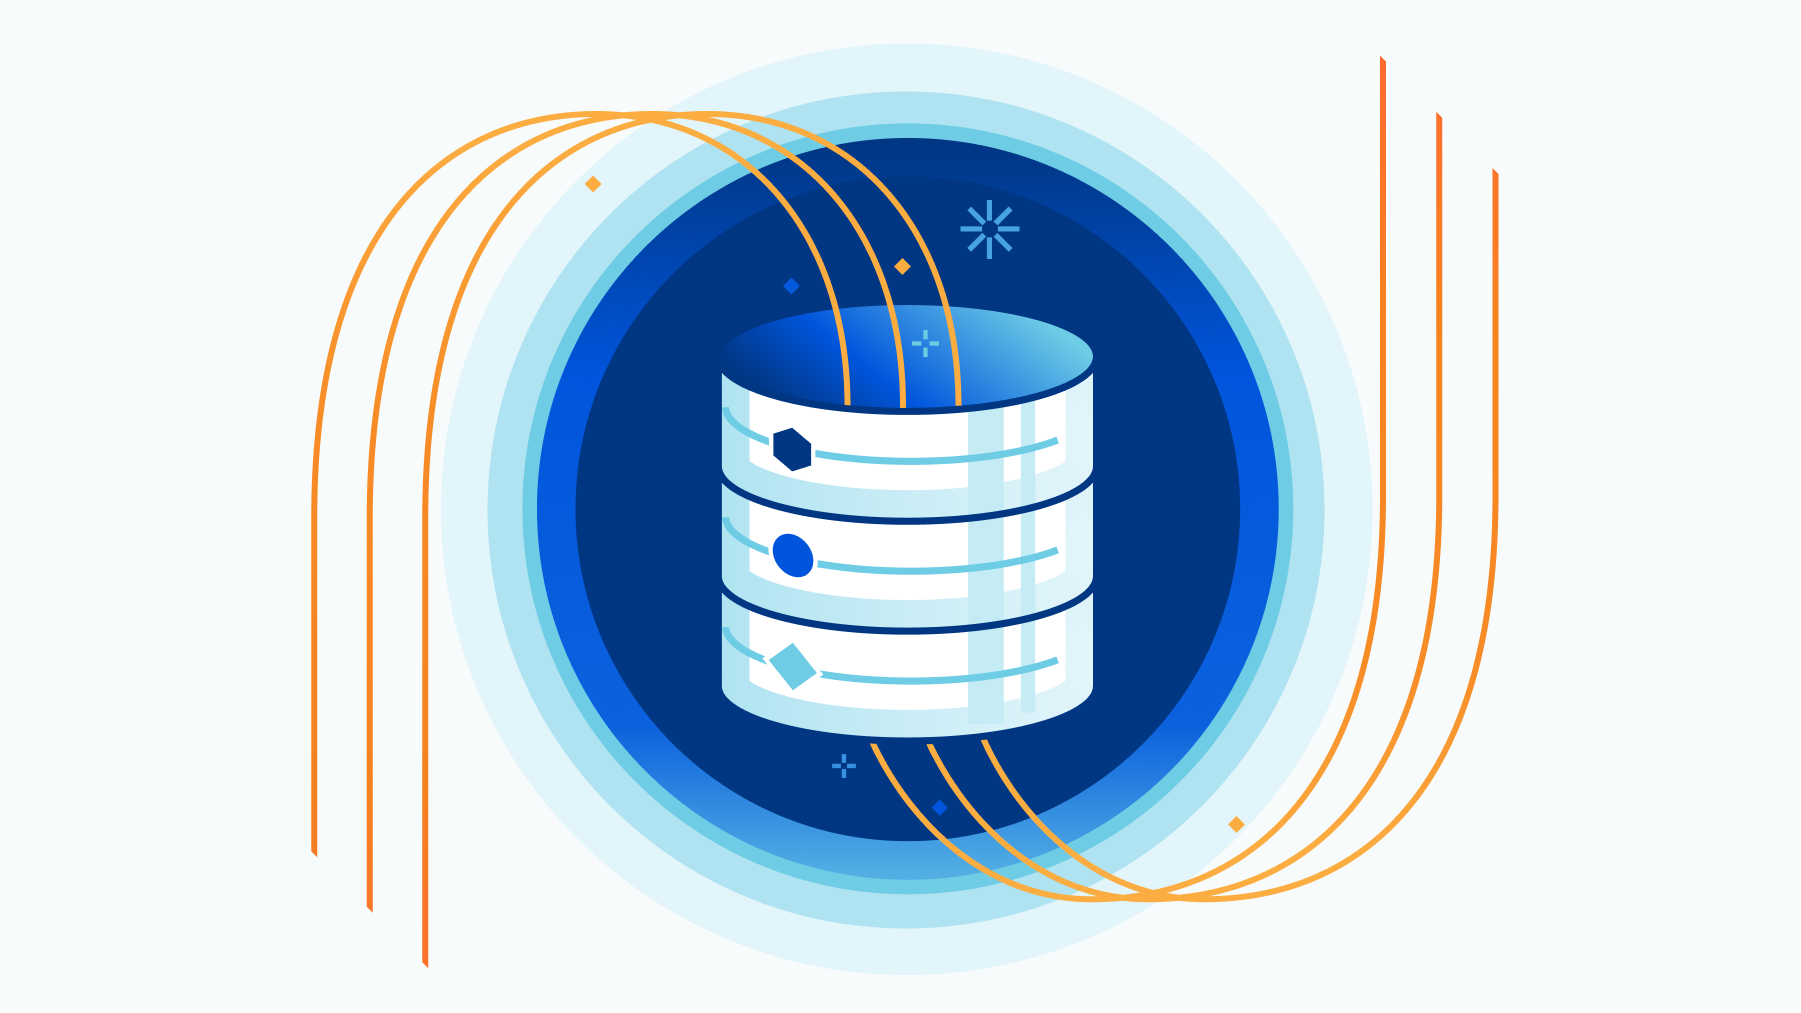
\includegraphics[height=0.7\paperheight]{cover}
    % \end{picture}    
    % }}
\usebackgroundtemplate{
  \tikz[overlay,remember picture] 
  \node[opacity=0.3, at=(current page.south east),anchor=south east, yshift=2cm,xshift=2cm] {
    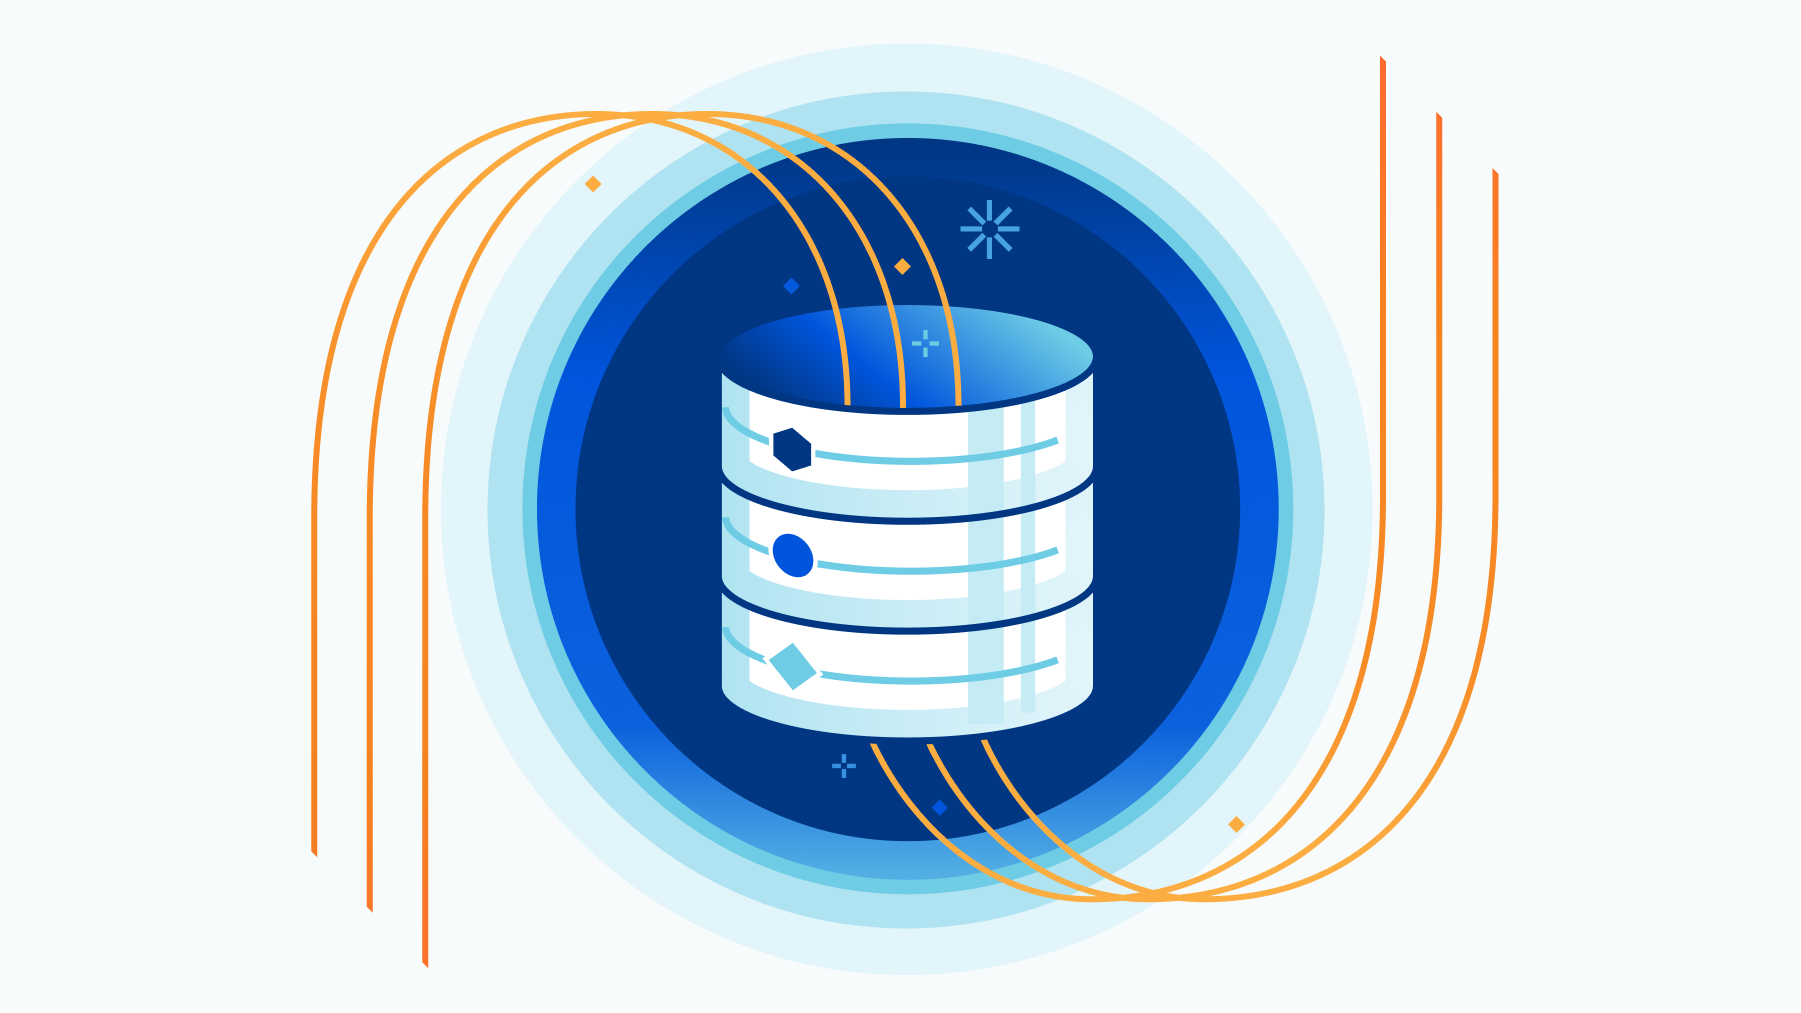
\includegraphics[height=0.6\paperheight]{cover}};
}
    \begin{frame}
        \section{\textcolor{darkmidnightblue}{关于课程}}
    \end{frame}
}

\begin{frame}
    \frametitle{关于课程}
\begin{block}{数据库}
    \alert{数据库}是计算机、软件工程、数据科学等专业的核心课程。

它向上能支撑互联网、银行等不同行业的应用,向下能触及存储、查询优化、编译、分布式计算等计算机核心技术。
\end{block}
\grid{顶} \grid{天} \grid{立} \grid{地}
\end{frame}


\begin{frame}
    \frametitle{预备知识}    
原则上几乎不需要预备知识,掌握\alert{阅读文档}(尤其是英文文档)和\alert{安装软件}地能力即可。
\pause
\begin{block}{重点}
本课程是应用导向的,因此存储、查询优化、事务等技术几乎不涉及。重点是:
\begin{itemize}
    \item  如何使用数据库
    \item  如何设计数据库
\end{itemize}
    
\end{block}
\end{frame}

\begin{frame}[fragile]
\begin{center}
    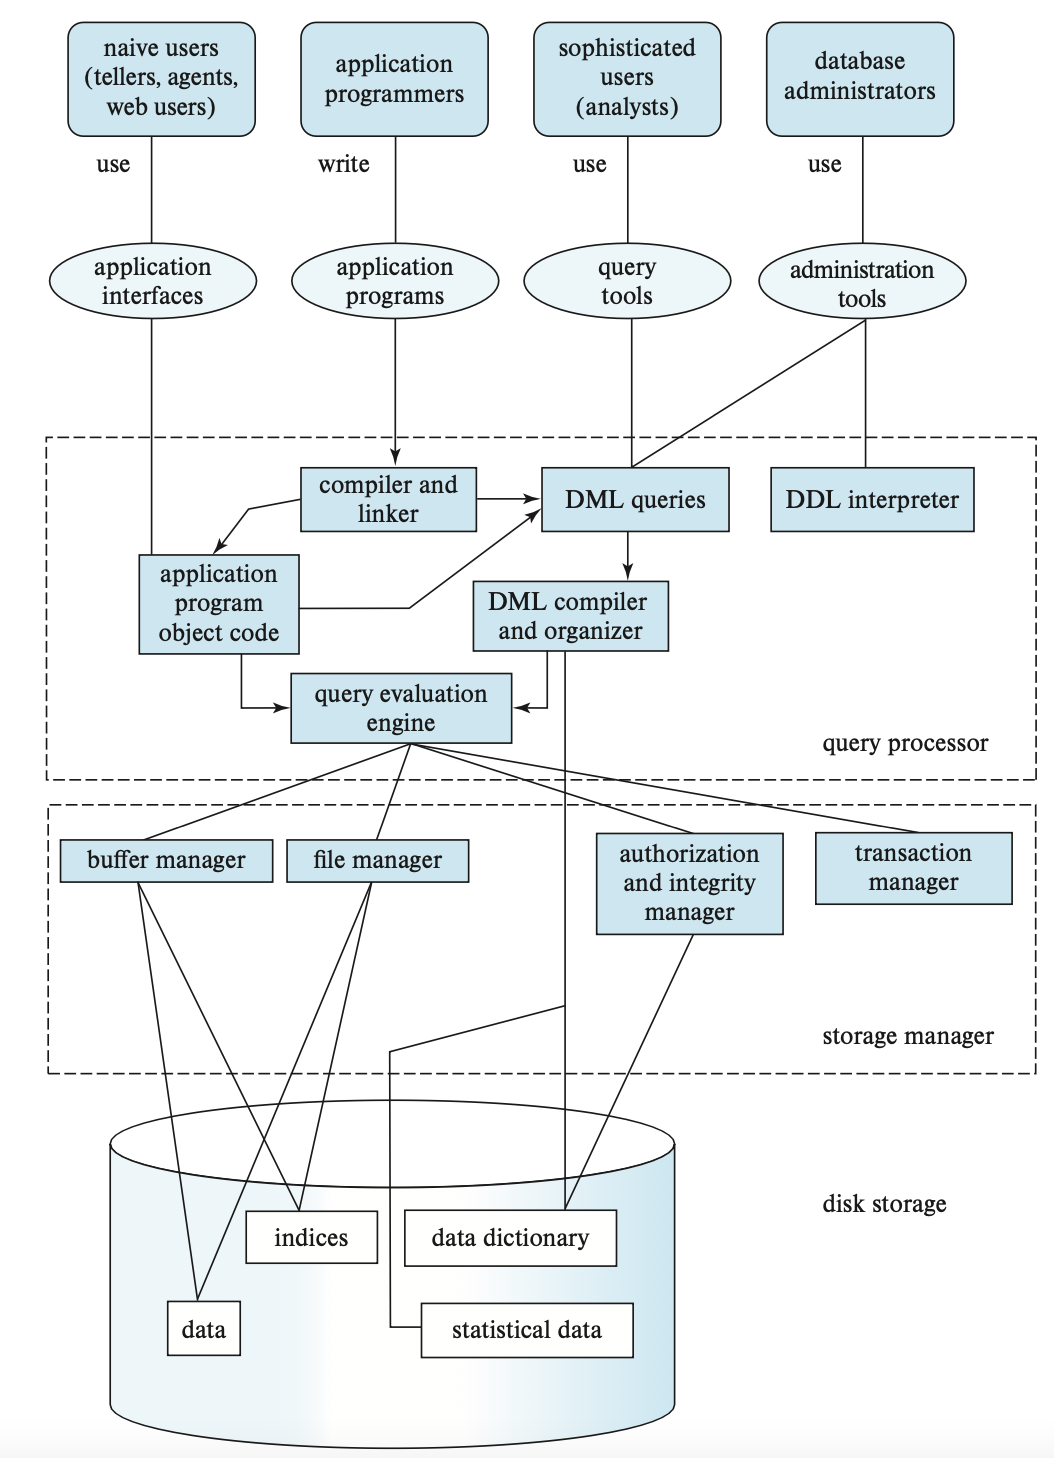
\includegraphics[height=\paperheight]{DBMS}
\end{center}
\end{frame}

\begin{frame}
    \frametitle{参考书籍}
    \href{https://book.douban.com/subject/30345517/}{Database System Concepts}, 7th edition, by Abraham Silberschatz, Henry F Korth, and S Sudarshan.
    \begin{center}
        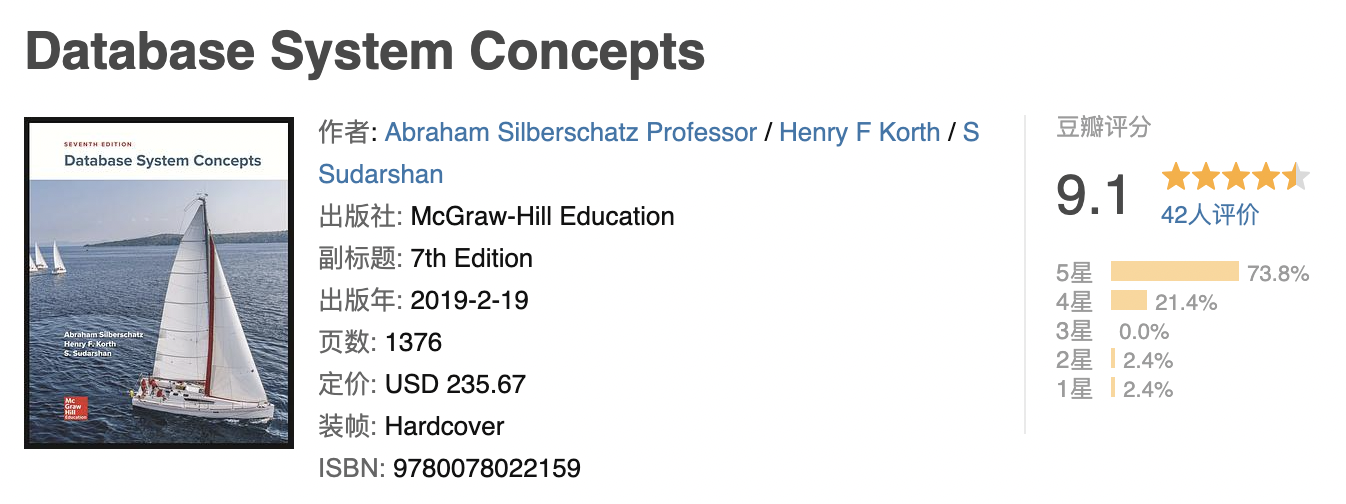
\includegraphics[height=.5\paperheight]{image/dsc-book}
    \end{center}
\end{frame}

\begin{frame}
    \frametitle{课程资源}
    \begin{columns}
        \column{0.475\textwidth} 
        \begin{itemize}
            \item 代码及作业@\href{https://github.com/ChenZhongPu/db-swufe}{GitHub}
            \item Slides@\href{https://zhongpu.info/teaching/cs205-2022-fall/}{Zhongpu.info}
            \item 作业提交@飞书 (\small 扫描后加入企业,点击\alert{「切换企业」},再扫描一次)
        \end{itemize}
        \column{0.475\textwidth} 
        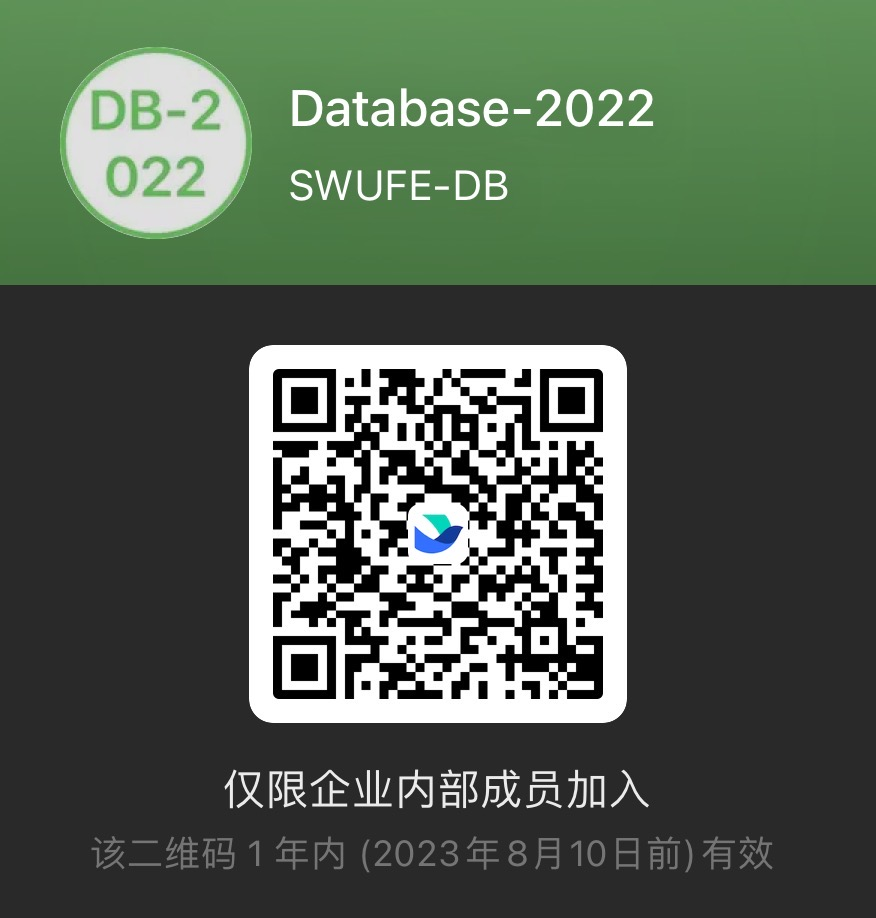
\includegraphics[height=0.85\paperheight]{image/feishu}
    \end{columns}
\end{frame}

\begin{frame}
    \frametitle{评价标准}
    
    \begin{tikzpicture}
        \colorlet{good}{green!75!black}
        \colorlet{bad}{red}
        \colorlet{neutral}{black!60}
        \colorlet{none}{blue!75!black}
      
        \node[align=center,text width=3cm]{考核};
      
        \begin{scope}[line width=4mm,rotate=270]
          \draw[good]          (180:2cm) arc (180:324:2cm);
          \draw[neutral]       (-36:2cm) arc (-36:0:2cm);
          \draw[bad]  (0:2cm)  arc (0:108:2cm);
          \draw[none] (108:2cm) arc (108:180:2cm);
      
          \newcount\mycount
          \foreach \angle in {0,72,...,3599}
          {
            \mycount=\angle\relax
            \divide\mycount by 10\relax
            \draw[black!15,thick] (\the\mycount:18mm) -- (\the\mycount:22mm);
          }
      
          \draw (0:2.2cm) node[below] {平时表现 (10\%)};
          \draw (-90:2.2cm) node[left] {作业 (40\%)};
          \draw (65:2.2cm) node[right] {期末考试 (30\%)};
          \draw (130:2.2cm) node[right] {Project (20\%)};
        \end{scope}
        % \draw[gray] (0,0) circle (2.2cm) circle (1.8cm);
      \end{tikzpicture}
      \begin{tikzpicture}
        \node[fill=red!80, text=white, blur shadow={shadow xshift=-0.5ex},
        text width=8em,anchor=south west,rounded corners, ]
        {严禁抄袭!
        };
      \end{tikzpicture}
\end{frame}
\begin{frame}
    \frametitle{软件工具}    
    PostgreSQL 14: \emph{The World's Most Advanced Open Source Relational Database}

    
\includegraphics[width=.9\paperwidth]{image/pg-home}
\end{frame}

\begin{frame}
\href{https://db-engines.com/en/ranking}{DB-Engines Ranking} 

\begin{table}
    \caption{DB Rank}
    \begin{tabular}{lll}
      \toprule
      Rank & DBMS & Database Model \\
      \midrule
      1 & \textcolor{blue}{Oracle} & Relational \\
      2 & \textcolor{blue}{MySQL} & Relational \\
      3 & \textcolor{blue}{SQL Server} & Relational \\
      4 & \textcolor{blue}{PostgreSQL} & Relational \\
      5 & \textcolor{blue}{MongoDB} & Document \\
      6 & \textcolor{blue}{Redis} & Key value \\
      \bottomrule
    \end{tabular}
\end{table}
\end{frame}

\begin{frame}
    
\includegraphics[width=.9\paperwidth]{image/pg-mysql1}
    \begin{itemize}
        \item 会什么选什么。PG 功能强大,但是我只会玩 MySQL 所以我用 MySQL 。
        \item 选 mysql,用 pg 的人一般不会有这个疑问。
    \end{itemize}
\end{frame}

\begin{frame}
    \frametitle{软件工具}    
\href{https://www.jetbrains.com/datagrip/}{DataGrip},Navicat,pgAdmin,...

\begin{center}
    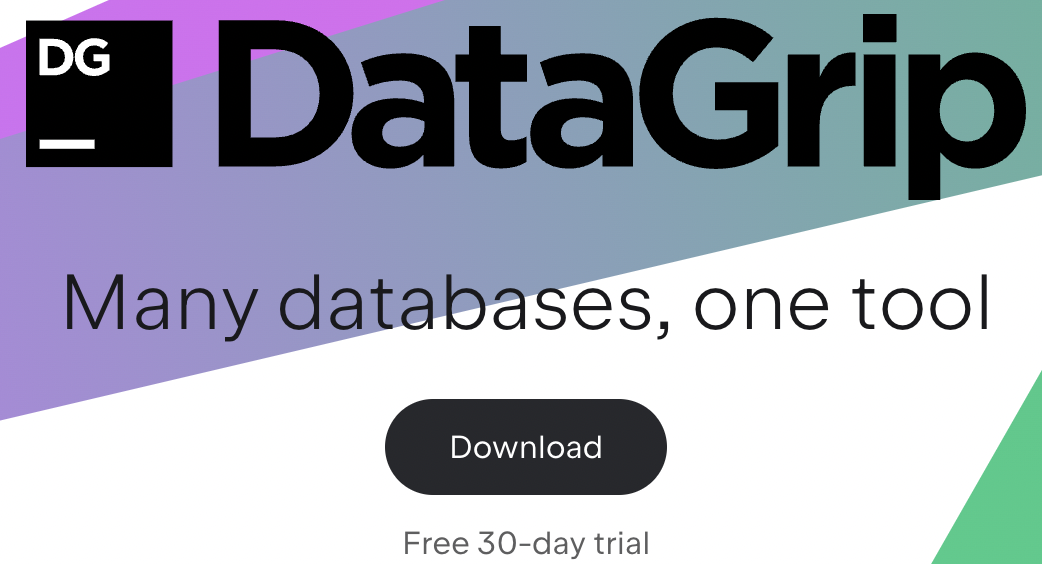
\includegraphics[width=.55\paperwidth]{image/datagrip}
\end{center}

\end{frame}
\end{document}